\section{FORS+C}
FORS (Forest of Random Subsets) is a few-time signature scheme used at the bottom of the stateless hypertree \cite{sphincsplus_paper2019}. FORS allows to sign a limited number of messages, when the security degrades with each use. Standard FORS signs a message by revealing \texttt{k} secret values, one from each of \texttt{k} binary trees of height \texttt{a}. The message digest determines which leaf to reveal from each tree. FORS+C \cite{wotsc_sphincsc2022} applies the similar grinding optimization as WOTS+C: by searching for a digest where the last tree's index equals 0, the authentication path and leaf for that tree can be omitted entirely from the signature.

\subsection{FORS Structure}
FORS consists of \texttt{k} binary trees, each of height \texttt{a}:
\begin{itemize}
    \item Each tree has \texttt{$2^a$} leaves
    \item Each leaf is derived from \texttt{SK.seed} using PRF with address type \texttt{FORS\_PRF}
    \item The message digest is split into \texttt{k} chunks of \texttt{a} bits each
    \item Each chunk selects one leaf index from the corresponding tree
\end{itemize}
\begin{figure}[h!]
    \centering
    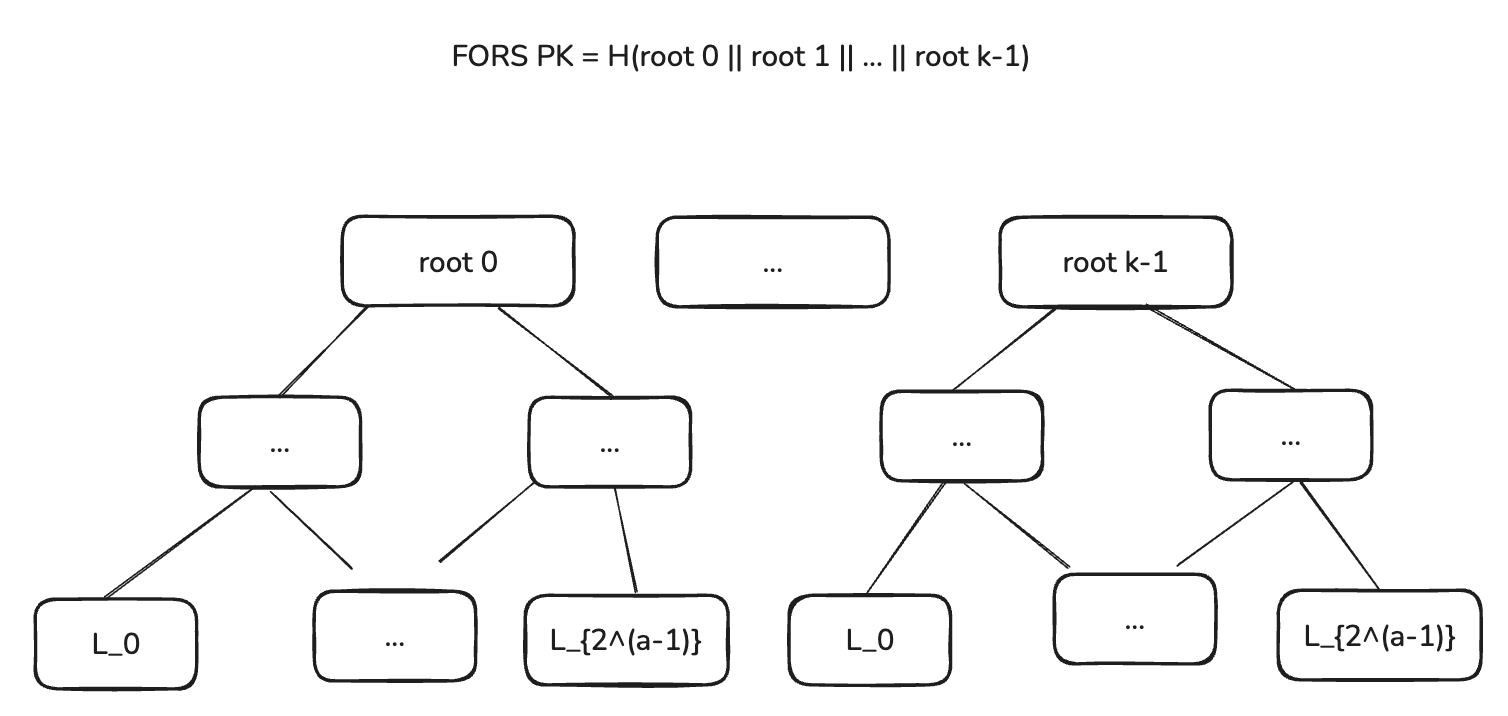
\includegraphics[width=0.8\linewidth]{content/img/fors.png}
    \caption{FORS architecture}
    \label{fig:shrincs}
\end{figure}
The FORS public key is the tweakable hash of the tree roots. With the +C grinding optimization, the last tree's root is excluded: \texttt{FORS+C PK = Tw(PK.seed, ADRS, root\_0 || ... || root\_{k-2})}, using address type \texttt{FORS\_PK}. The last tree is not needed in the public key computation since grinding guarantees the last index is always 0.

\subsection{Grinding Condition}
FORS+C uses the single-phase message hash \texttt{H\_msg\_fors} (Section~5.4.2):
\begin{verbatim}
    digest = H_msg_fors(ADRS, R, PK.seed, PK.root, m)
    condition: digest[last a bits] == 0
\end{verbatim}

The signer searches for an \texttt{R} that satisfies this condition by iterating a counter inside \texttt{PRF\_msg\_ctr} (Section~5.3). Each counter value produces a fresh \texttt{R}, which is then evaluated via \texttt{H\_msg\_fors}. The verifier only sees the final \texttt{R} that satisfied the condition.

Expected grinding cost is $\approx 2^a$ iterations. With \texttt{a = 22}, this is approximately 4 million iterations. Each iteration requires one HMAC-SHA-256 (for \texttt{PRF\_msg\_ctr}) plus one SHA-256 (for \texttt{H\_msg\_fors}).

\subsection{Message to Indices}
The \texttt{fors\_msg\_to\_indices} function converts a message digest into \texttt{k} leaf indices, one for each FORS tree. Each index is extracted as a consecutive a-bit chunk from the digest. The indices are integers in the range \texttt{[0, 2\string^a - 1]}.
\begin{verbatim}
    Algorithm: fors_msg_to_indices(digest)
    Input:
        digest: message digest
    Output:
        indices: array of k integers in [0, 2^a - 1]

    1. indices ← []
    2. for i from 0 to k - 1:
        a. indices[i] ← extract_bits(digest, i * a, a)
    3. return indices
\end{verbatim}

\paragraph{Note:} \texttt{extract\_bits(x, offset, length)} extracts length bits from byte string \texttt{x} starting at bit position offset, returned as an unsigned integer. Bits are numbered in big-endian order: bit \texttt{0} is the most significant bit of byte \texttt{x[0]}.
\paragraph{Note:} The message digest also encodes which FORS instance is used, as determined by the tree and leaf indices parsed from the stateless signature digest (Section~10.5). The output size of \texttt{H\_msg\_fors} must be sufficient to encode all \texttt{k} indices: at least \texttt{roundup((k*a) / 8)} bytes.

\subsection{Grinding}
The \texttt{fors\_grind} function searches for a counter value where the last tree's index equals 0. This eliminates the need to include the authentication path and leaf for tree \texttt{k-1} in the signature.
%\mknote{This can be variable. we can require one, two, or more indices to be 0. Also need to adapt the message hashing, and indices extraction.}
\begin{verbatim}
    Algorithm: fors_grind(m, SK.prf, PK.seed, PK.root, ADRS, opt_rand)
    Input:
        m: message
        SK.prf: PRF key for randomness
        PK.seed: public seed
        PK.root: public key root
        ADRS: tweak
        opt_rand: optional randomness (n bytes)
    Output:
        indices: array of k integers
        R: randomness that satisfied the grinding condition
        digest: the digest that satisfied the grinding condition

    1. setTypeAndClear(ADRS, SL_H_MSG)
    2. for ctr from 0 to 2^32 - 1:
        a. R ← PRF_msg_ctr(SK.prf, PK.seed, opt_rand, ctr, m)
        b. digest ← H_msg_fors(ADRS, R, PK.seed, PK.root, m)
        c. indices ← fors_msg_to_indices(digest)
        d. if indices[k-1] == 0:
            return (indices, R, digest)
    3. abort with error
\end{verbatim}

\subsection{Secret Key Generation}
The \texttt{fors\_SKgen} function derives a secret leaf value for a specific tree and leaf index. Each leaf's secret is deterministically generated using PRF with the tree index and leaf index encoded in the address structure via \texttt{FORS\_PRF}. This ensures all $2^a$ leaves across all \texttt{k} trees can be regenerated from \texttt{SK.seed} without storing them.
\begin{verbatim}
    Algorithm: fors_SKgen(SK.seed, PK.seed, ADRS, tree_idx, leaf_idx)
    Input:
        SK.seed: secret seed
        PK.seed: public seed
        ADRS: tweak
        tree_idx: tree index (0 to k-1)
        leaf_idx: leaf index within tree
    Output:
        sk: secret value

    1. setTypeAndClear(ADRS, FORS_PRF)
    2. setKeyPairAddress(ADRS, tree_idx)
    3. setTreeIndex(ADRS, leaf_idx)
    4. sk ← PRF(PK.seed, ADRS, SK.seed)
    5. return sk
\end{verbatim}

\subsection{TreeHash}
The \texttt{fors\_treehash} function recursively computes FORS subtree roots. At height 0 (leaf level), it generates the secret key and hashes it to produce the leaf node using address type \texttt{FORS\_HASH}. At higher levels, it recursively computes left and right children, then hashes their concatenation using \texttt{FORS\_TREE}. This function is used both for computing full tree roots and for generating individual sibling nodes needed in authentication paths.

\paragraph{Note:} The structure is analogous to \texttt{xmss\_treehash} (Section~7.2), with the difference being the leaf computation (FORS uses hashed secret keys rather than WOTS+C public keys).
\begin{verbatim}
    Algorithm: fors_treehash(SK.seed, PK.seed, ADRS, tree_idx, target_height, start_idx)
    Input:
        SK.seed, PK.seed: seeds
        ADRS: tweak
        tree_idx: tree index (0 to k-1)
        target_height: height of output node (0 = leaf level)
        start_idx: leftmost leaf index in subtree
    Output:
        node: hash value

    1. if target_height == 0:
        a. sk ← fors_SKgen(SK.seed, PK.seed, ADRS, tree_idx, start_idx)
        b. setTypeAndClear(ADRS, FORS_HASH)
        c. setKeyPairAddress(ADRS, tree_idx)
        d. setTreeHeight(ADRS, 0)
        e. setTreeIndex(ADRS, start_idx)
        f. return Tw(PK.seed, ADRS, sk)
    2. left ← fors_treehash(SK.seed, PK.seed, ADRS, tree_idx, 
                                    target_height - 1, start_idx)
    3. right ← fors_treehash(SK.seed, PK.seed, ADRS, tree_idx, 
            target_height - 1, start_idx + 2^(target_height - 1))
    4. setTypeAndClear(ADRS, FORS_TREE)
    5. setKeyPairAddress(ADRS, tree_idx)
    6. setTreeHeight(ADRS, target_height)
    7. setTreeIndex(ADRS, start_idx >> target_height)
    8. return Tw(PK.seed, ADRS, left || right)
\end{verbatim}

\subsection{FORS Authentication path}
The \texttt{fors\_auth\_path} function generates the a sibling nodes needed to authenticate a revealed leaf up to its tree root. At each height h, the sibling is the node that, when combined with the current path node, produces the parent. The sibling index is computed by XORing the leaf index with \texttt{2\string^h}, which flips the h-th bit to identify the sibling's subtree.
\begin{verbatim}
    Algorithm: fors_auth_path(SK.seed, PK.seed, ADRS, tree_idx, leaf_idx)
    Input:
        SK.seed, PK.seed: seeds
        ADRS: tweak
        tree_idx: tree index (0 to k-1)
        leaf_idx: leaf index being revealed
    Output:
        auth: authentication path (a * n bytes)

    1. auth ← []
    2. for h from 0 to a - 1:
        a. sibling_start ← (leaf_idx XOR 2^h) AND (0xFFFFFFFF << h)
        b. auth ← auth || fors_treehash(SK.seed, PK.seed, ADRS, tree_idx, h, sibling_start)
    3. return auth
\end{verbatim}

\subsection{Signature generation}
The \texttt{fors\_sign} function produces a FORS+C signature. Due to grinding, the last tree's index is guaranteed to be 0, so tree \texttt{k-1} is entirely excluded from the signature. The signature reveals \texttt{k-1} leaves with their authentication paths. Signature format: \texttt{R || (sk\_0 || auth\_0) || ... || (sk\_{k-2} || auth\_{k-2})}
\begin{verbatim}
    Algorithm: fors_sign(m, SK.seed, SK.prf, PK.seed, PK.root, ADRS)
    Input:
        m: message
        SK.seed: secret seed
        SK.prf: PRF key
        PK.seed: public seed
        PK.root: public key root
        ADRS: tweak
    Output:
        sig: FORS+C signature
        digest: the digest that satisfied the grinding condition

    1.  opt_rand ← random(n) or PK.seed
    2.  (indices, R, digest) ← fors_grind(m, SK.prf, PK.seed, PK.root, ADRS, opt_rand)
    3.  (tree_idx, leaf_idx) ← parse_idx(digest)
    4.  setLayerAddress(ADRS, 0)
    5.  setTreeAddress(ADRS, tree_idx[0] * 2^h_prime + leaf_idx[0])
    6.  sig ← R
    7.  for i from 0 to k - 2:
        a. sk_i ← fors_SKgen(SK.seed, PK.seed, ADRS, i, indices[i])
        b. auth_i ← fors_auth_path(SK.seed, PK.seed, ADRS, i, indices[i])
        c. sig ← sig || sk_i || auth_i
    8.  return (sig, digest)
\end{verbatim}

\subsection{Public Key Recovery}
The \texttt{fors\_pkFromSig} function recovers the FORS+C public key from a signature. For each of the first \texttt{k-1} trees, it hashes the revealed secret key to obtain the leaf, then iteratively combines with authentication path nodes to compute the tree root. The FORS+C public key is the tweakable hash of these \texttt{k-1} roots (tree \texttt{k-1} is excluded entirely due to grinding). The function returns \texttt{"false"} if the grinding condition is not satisfied.
\begin{verbatim}
    Algorithm: fors_pkFromSig(sig, indices, PK.seed, ADRS)
    Input:
        sig: FORS+C signature (R || sk/auth pairs)
        indices: pre-computed array of k FORS leaf indices
        PK.seed: public seed
        ADRS: tweak
    Output:
        pk: FORS+C public key or "false" if invalid
    
    1.  roots ← []
    2. if indices[k-1] != 0:
        return false
    3.  offset ← R_SIZE     // skip R (already consumed by caller)
    4.  for i from 0 to k - 2:
        a. sk_i ← sig[offset : offset + n]
        b. auth_i ← sig[offset + n : offset + n + a * n]
        c. offset ← offset + n + a * n
        d. setTypeAndClear(ADRS, FORS_HASH)
        e. setKeyPairAddress(ADRS, i)
        f. setTreeHeight(ADRS, 0)
        g. setTreeIndex(ADRS, indices[i])
        h. node ← Tw(PK.seed, ADRS, sk_i)
        i. idx ← indices[i]
        j. for h from 0 to a - 1:
               setTypeAndClear(ADRS, FORS_TREE)
               setKeyPairAddress(ADRS, i)
               setTreeHeight(ADRS, h + 1)
               setTreeIndex(ADRS, idx >> 1)
               if (idx AND 1) == 0:
                   node ← Tw(PK.seed, ADRS, node || auth_i[h * n : (h + 1) * n])
               else:
                   node ← Tw(PK.seed, ADRS, auth_i[h * n : (h + 1) * n] || node)
               idx ← idx >> 1
        k. roots[i] ← node
    5.  setTypeAndClear(ADRS, FORS_PK)
    6.  pk ← Tw(PK.seed, ADRS, roots[0] || ... || roots[k-2])
    7.  return pk
\end{verbatim}